\documentclass[11pt,letterpaper]{article}
\usepackage[utf8]{inputenc}
\usepackage{graphicx, geometry, amsmath, amssymb, url, booktabs, xcolor, listings, tabularx, array}
\usepackage[numbers,sort&compress]{natbib}
\usepackage{hyperref}
\usepackage{xurl}
\geometry{margin=1in}
\hypersetup{colorlinks=true, linkcolor=black, citecolor=black, urlcolor=black}
\renewcommand{\topfraction}{0.9}
\renewcommand{\bottomfraction}{0.8}
\renewcommand{\textfraction}{0.07}
\renewcommand{\floatpagefraction}{0.75}
\newcolumntype{Y}{>{\raggedright\arraybackslash}X}
\newcommand{\Astar}{A$^{*}$}
\setlength{\emergencystretch}{2em}

\title{Steering a 3B Code Model Selects One Known Algorithm Rather Than Diversifying}
\author{}
\date{}
\makeatletter
\renewcommand{\@maketitle}{\newpage\null\vskip 1em\begin{center}{\LARGE \@title \par}\end{center}\par\vskip 1.5em}
\makeatother

\begin{document}
\maketitle

\begin{abstract}
Temperature, prompt instructions and activation steering are used to make language models propose less obvious solutions, but it is rarely tested whether they change the solution idea or only its wording. We label the algorithm family of every program Qwen2.5-3B-Instruct writes for open sorting and path search prompts, execute each program, and test whether a difference-in-means steering direction away from the default family flattens the distribution over families or selects one alternative. In a preregistered test whose rules, strengths and predicted gainers were frozen by hash, the direction met the selection rule on both tasks, replicated on a redraw with fresh seeds. On sorting in that redraw, bubble sort fell from 62\% of programs to 0\%, quicksort rose to 68\%, and the entropy over families lay 0.73 bits below the mean of five random directions of matched norm (95\% CI [$-0.95$, $-0.45$]). The scope is narrow: one 3B model, one bare prompt per task, a rule that accepted the top prediction of either of two frozen rankings, and random directions that alone move sorting substantially. On path search \Astar{} replaced breadth first search but the pass rate halved, missing the frozen correctness bar. Selection does not reach new ideas: steering toward families the model never writes fails where naming them in the prompt succeeds, and every passing program outside the labelled families that a blind judge checked was a known algorithm. Temperature adds families slowly while correctness collapses, and random seed strings concentrate the choice. On these tasks, the controls choose among known ideas; they do not create new ones.
\end{abstract}

\section{Introduction}
\label{sec:intro}

Language models are increasingly asked to design solutions rather than to recall them, and users who want a less obvious design reach for two kinds of control. The first is decoding: raising the sampling temperature is widely treated as the model's creativity parameter \citep{Peeperkorn2024}, although high temperatures also degrade text \citep{Holtzman2019}. The second is the model's internal state: activation steering adds a direction to the residual stream during generation \citep{Turner2023,Rimsky2024}, and recent work steers models toward more creative or more diverse outputs \citep{Olson2024,Zhu2026,Khanh2025}. Both kinds of control are usually judged by how different the outputs look. For a design task, the question that matters is narrower: does the control make the model pick a different solution idea, and is that idea one it did not already have?

Code generation lets us ask that question with exact measurements. Asked to \emph{implement a path search algorithm}, a chat model writes breadth first search (BFS) most of the time, with depth first search (DFS), Dijkstra's algorithm and \Astar{} search as a minority. Every program can be labelled with the algorithm family it implements and executed against a fixed test suite. A control that adds novelty should move probability onto families the model rarely writes, or onto programs no label covers, while those programs still pass. Instruction tuning is known to narrow output diversity \citep{Kirk2023,Padmakumar2023,Zhang2025}, and incidental prompt cues are known to move which algorithm family a code model picks \citep{Narula2026}. What is missing is a controlled test of how internal edits move this choice, and against which baseline.

The baseline is the hard part. A steering vector of the right norm changes outputs whatever its direction, and the effect of a single random direction varies widely from draw to draw. A targeted direction that raises diversity once is therefore weak evidence. A cleaner test separates two behaviours that a diversity score conflates. A \emph{flattening} intervention spreads probability across the families the model knows, so the share of the default falls and no other family takes over. A \emph{selecting} intervention hands most of the mass to one other family. The two predict opposite things for entropy relative to random directions of the same norm, and only selection predicts which family will gain.

We ran that test as a preregistered experiment on Qwen2.5-3B-Instruct \citep{Yang2024}, on two open coding prompts (path search and sorting), with decision rules frozen by hash before the data existed. We build a steering direction from the difference in means between activations of programs that do and do not implement the model's default family, add it to the residual stream during generation, and compare it with five random directions of matched norm, the corresponding direction of the other task, temperature, and simply asking for a family. We call it the \emph{direction away from the mode}. The direction meets the frozen selection rule on both tasks, on the main draw and on a redraw with fresh seeds. On sorting in the redraw, bubble sort falls from 62\% of programs to 0\% and quicksort, the top prediction of the frozen projection ranking, rises to 68\%, while the entropy of the distribution over algorithm families falls 0.73 bits below the random direction mean (95\% CI [$-0.95$, $-0.45$]; Figure~\ref{fig:hero}). The scope of this result is one 3B model and one bare prompt per task, and the rule accepted the top prediction of either of two frozen rankings. The same pattern holds on a menu of two families in a second experiment under a different prompt. Selection does not reach new ideas: steering toward families the model never writes mostly fails where naming them in the prompt succeeds, and every passing program outside the labelled families that a blind judge checked (70 of 70) was a known algorithm. Temperature, random seed strings and negative instructions in the prompt behave the same way at the level of behaviour: they reorder or concentrate a small menu of textbook ideas.

Our contributions are:
\begin{itemize}
  \item \textbf{A preregistered test of selecting against flattening for activation steering}, with frozen predictions of the gaining family and a random direction baseline averaged over draws (Section~\ref{sec:method}).
  \item \textbf{Evidence that steering selects, preregistered and replicated across draws and tasks on one model.} On a redraw with fresh seeds the direction away from the mode gives quicksort 68\% and \Astar{} 63\% of programs, against 24\% and 6\% under random directions of matched norm. On sorting, entropy falls 0.73 bits below the random mean [$-0.95$, $-0.45$], and on path search the nonmodal share rises 0.53 above it [0.45, 0.60] (Section~\ref{sec:res-select}). A second, exploratory experiment with a different prompt and layer band turns 29\% DFS into 97\% DFS at an unchanged pass rate (Section~\ref{sec:res-twofam}).
  \item \textbf{A prompting ceiling for novelty.} Steering toward families absent from the baseline produces them in 0\% to 1.3\% of programs for three of four targets, while naming them in the prompt produces them in 92\% to 100\%; all 70 passing programs outside the labelled families that a blind judge checked were known algorithms (Section~\ref{sec:res-offmenu}).
  \item \textbf{Behavioural context for the same conclusion.} From $T = 0.3$ to $T = 1.0$, temperature adds 0.4 (path search) and 1.8 (sorting) expected families per ten programs while the path search pass rate falls from 0.49 to 0.19. Random seed strings lower the entropy over families by 0.34 and 0.68 bits. Negative instructions against families the model never writes reshuffle the families it does write, violating regularity in 8 of 46 tested cells against 0 of 45 for placebo prompts (Sections~\ref{sec:res-temp} and~\ref{sec:res-context}).
\end{itemize}

Section~\ref{sec:related} places this work against prior studies of temperature, steering and negative instructions; Sections~\ref{sec:method} and~\ref{sec:setup} give the method and setup, Section~\ref{sec:results} the results, and Sections~\ref{sec:discussion} to~\ref{sec:conclusion} discuss what they imply and where they stop.

\begin{figure}[!htbp]
  \centering
  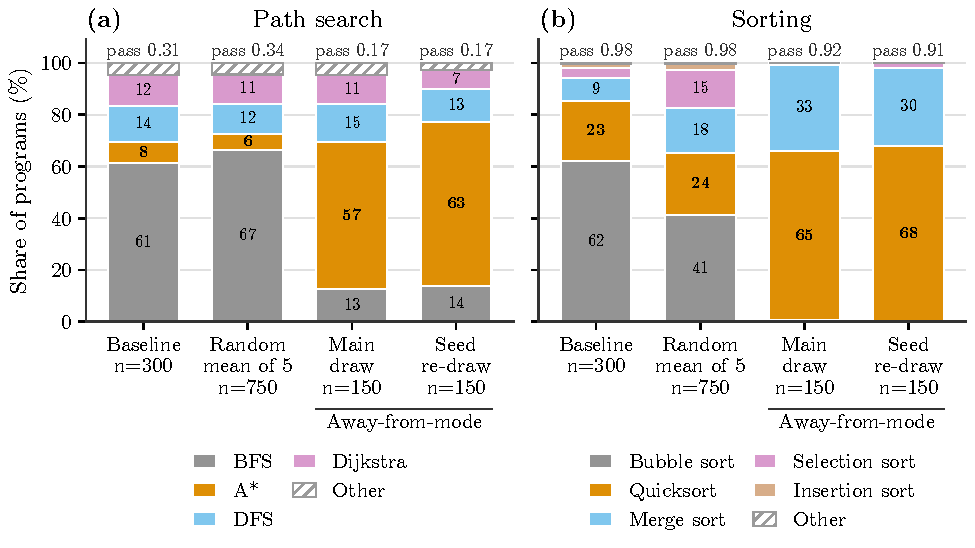
\includegraphics[width=\linewidth,height=0.85\textheight,keepaspectratio]{figures/fig1_v0.pdf}
  \caption{Share of programs implementing each algorithm family for Qwen2.5-3B-Instruct at temperature 0.7, on the bare path search prompt (a) and the bare sorting prompt (b). Each 100\%-stacked bar is one condition: the unsteered baseline ($n=300$); the pooled mean of five random directions of matched norm at the frozen strength $s_2$ ($n=750$); and the direction away from the mode at $s_2$ on the main draw and on a redraw with fresh seeds ($n=150$ each); we call this direction away-from-mode in the plot labels. The default family (BFS, bubble sort) is grey and the family predicted by the frozen projection ranking (A*, quicksort) is amber. Other named families are in muted colours; the hatched white segment pools all remaining labels. Numbers inside segments are shares in percent, shown for segments of at least 5\%. The number above each bar is the oracle pass rate. The direction away from the mode moves most of the default's share to the predicted family on both tasks and both seed draws: A* rises from 8\% to 57\% and 63\%, and quicksort from 23\% to 65\% and 68\%, while bubble sort falls to 1\% and 0\%. Random directions of the same norm leave BFS in place on path search (61\% vs.\ 67\%). On sorting they reduce bubble sort to 41\%, spreading the freed share over merge and selection sort, and leave quicksort at 24\%. On path search, selection comes with a lower pass rate (0.31 to 0.17); on sorting the pass rate stays above 0.9.}
  \label{fig:hero}
\end{figure}

\section{Related Work}
\label{sec:related}

\paragraph{Temperature, sampling and output diversity.} \citet{Peeperkorn2024} find that temperature is weakly correlated with novelty and moderately correlated with incoherence in story generation, and \citet{Holtzman2019} show that unrestricted sampling at high temperature degenerates. Instruction tuning and RLHF reduce output diversity \citep{Kirk2023}, writing with a model homogenises content \citep{Padmakumar2023}, and NoveltyBench finds that models produce far fewer distinct answers than humans \citep{Zhang2025}. For code, \citet{Narula2026} report that subtle prompt cues shift which algorithm family a model implements. These studies measure diversity in text or embeddings. We measure it as the distribution over algorithm families checked by execution and separate the number of ideas from the number of phrasings of each, so that a control that rewrites the same idea is not credited with a new one.

\paragraph{Activation steering and its reliability.} Adding a direction to the residual stream steers behaviour \citep{Turner2023,Zou2023}. Contrastive Activation Addition builds the direction from the difference in means between contrasting examples \citep{Rimsky2024}, Inference-Time Intervention shifts selected attention heads along probe directions \citep{Li2023}, and a single difference-in-means direction mediates refusal \citep{Arditi2024}. These results rest on the view that concepts are encoded linearly \citep{Park2023}. Closest to our setting, difference-in-means directions added during generation push code models toward a target programming language or library, often against the prompt's request \citep{Rahman2026}. Reliability is uneven: steerability varies across inputs and some concepts resist steering \citep{Tan2024}, steering is unreliable when the target behaviour is not represented by a coherent direction \citep{Braun2025}, and simple prompting baselines often match or beat steering \citep{Wu2025}. Creativity steering adds the difference between creative and boring activations as a direction \citep{Olson2024}, while STARS and Riemannian activation steering optimise several directions jointly across concurrent generations to diversify them \citep{Zhu2026,Khanh2025}. Entropic activation steering raises the entropy of an agent's action distribution, and a shuffled steering vector of the same statistics leaves it unchanged \citep{Rahn2024}. Our test differs in three ways. The target is the algorithm family, checked by execution, rather than a language, library, action or style. It uses one fixed direction and asks whether that direction flattens or selects, with a frozen prediction of the gaining family. It compares against the mean of five random directions of matched norm per strength, because a single random draw can move the output distribution as much as a targeted one.

\paragraph{Negative instructions and choice structure.} Instruction steering adds the representation of an instruction to the forward pass \citep{Stolfo2024}, and negative constraints can backfire by priming the forbidden item \citep{Rana2026}. In the terms of discrete choice models, removing an option from a choice set should never lower the share of an option that remains; this property is called regularity, and its violations are a classic signature of context effects in human choice \citep{Huber1982}. Violations of related choice axioms have been reported for language models in economic settings \citep{Buchanan2026}. We use regularity as a test of whether a negative instruction in the prompt acts as restriction of the choice set, and we report it as context for the steering result rather than as a mechanism.

\section{Method}
\label{sec:method}

\subsection{Ideas, menus and the measurements on them}
\label{sec:measures}

For each prompt we sample programs, label each with the algorithm family it implements, and execute it. We call that family the program's \emph{idea}, and the set of ideas present in a prompt's baseline sample its \emph{menu}. The \emph{idea distribution} of a condition is the share of programs per idea, its \emph{mode} is the most frequent idea at baseline, and we define the \emph{nonmodal share} as one minus the share of the mode. Idea entropy is the Shannon entropy of the idea distribution in bits, with the Miller--Madow correction when conditions of different size are compared. For the question of ideas against phrasings, we report the expected number of distinct ideas and of distinct phrasings in a random draw of ten programs, a rarefaction of richness, the order-0 Hill number \citep{Hill1973}; two programs share a phrasing when their normalised code has edit distance similarity of at least 0.85. An idea outside the menu is a family absent from the menu. A program counts as correct only if it passes every test case of the execution oracle (Section~\ref{sec:setup}).

\subsection{The direction away from the mode}
\label{sec:direction}

Let $h_\ell(x)$ be the residual stream activation of program $x$ at layer $\ell$, averaged over a \emph{commitment window}: the 17 generated tokens starting at the first token that names or implements the idea, or the first 32 generated tokens when no such token exists. We define the direction away from the mode at layer $\ell$ as the difference in means
\begin{equation}
  v_\ell = \operatorname*{mean}_{x:\,\mathrm{idea}(x)\neq m} h_\ell(x) \;-\; \operatorname*{mean}_{x:\,\mathrm{idea}(x)=m} h_\ell(x),
\end{equation}
computed on baseline programs, where $m$ is the mode, and normalised to unit length. During generation we add $\alpha \cdot (\bar r_\ell / 3) \cdot v_\ell$ at each of the three band layers, where $\bar r_\ell$ is the median residual norm at that layer and $\alpha$ is the steering coefficient. The edit applies at the final prompt token and the first 64 generated tokens. The band (layers 32 to 34 of 36) was chosen by a linear probe for the idea at each layer, compared with a control task with shuffled labels \citep{Hewitt2019}; probe accuracy was nearly flat across layers, so the band choice carries little information. Figure~\ref{fig:method} summarises the construction and the comparators.

\begin{figure}[!htbp]
  \centering
  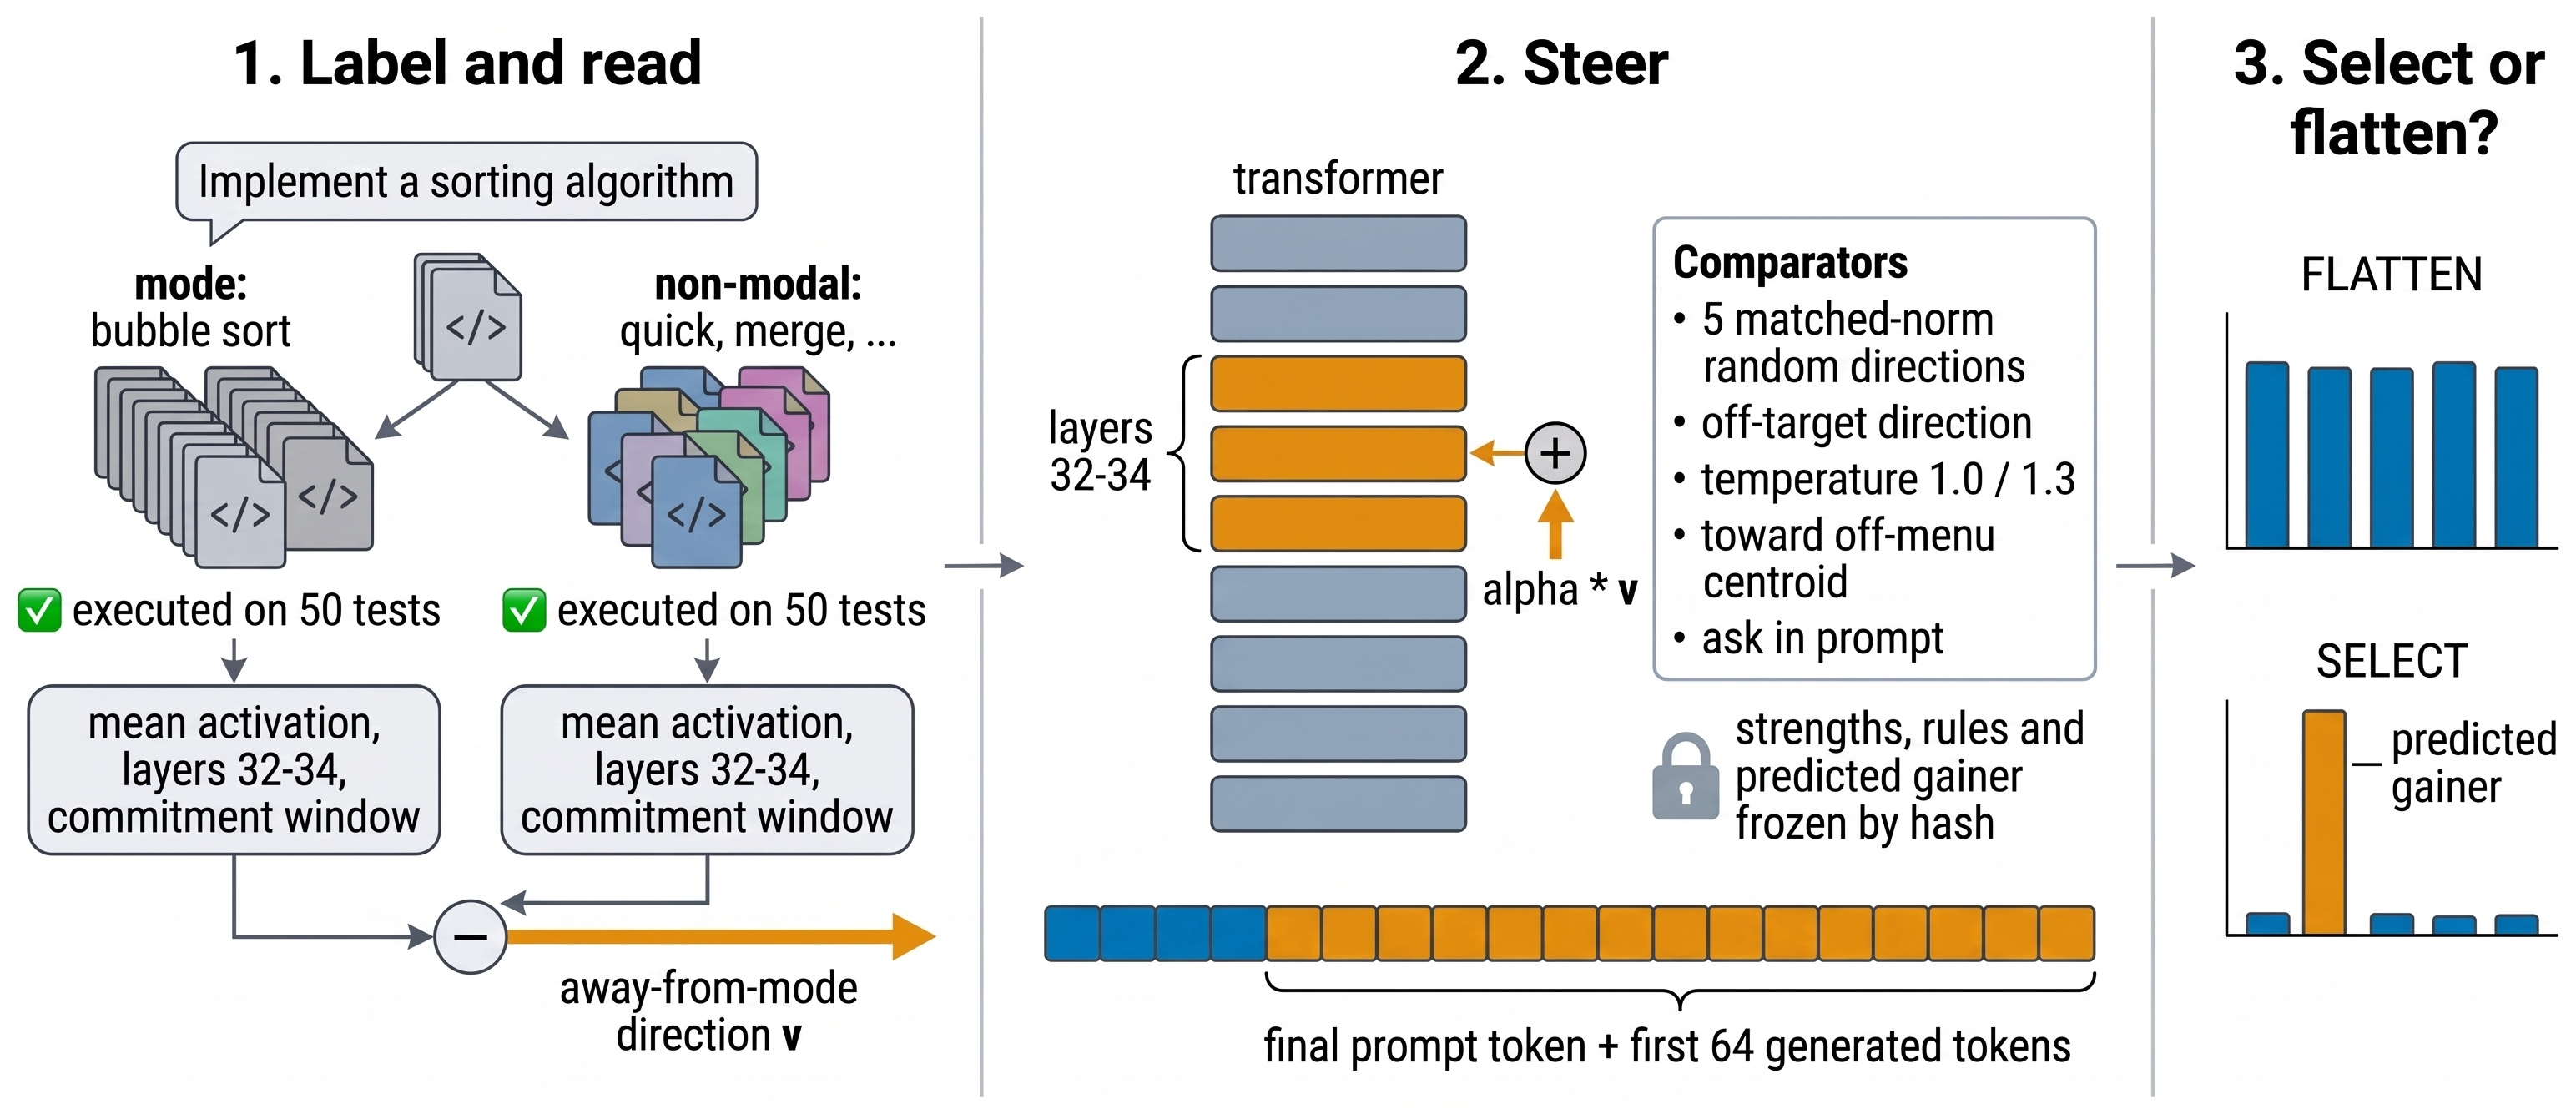
\includegraphics[width=\linewidth,height=0.85\textheight,keepaspectratio]{figures/fig2_v0.jpg}
  \caption{Schematic illustration of the method (no data). Left (\emph{Label and read}): programs sampled from the bare prompt \emph{Implement a sorting algorithm} are labelled by algorithm family and executed on 50 tests. Mean residual-stream activations over each program's commitment window at layers 32--34 are taken for the modal programs (bubble sort, grey) and the nonmodal programs (quick, merge, \ldots). Their difference gives $v$, the direction away from the mode (orange). Middle (\emph{Steer}): $\alpha v$ is added to layers 32--34 (orange blocks) at the final prompt token and the first 64 generated tokens (orange cells), at strengths frozen in advance together with the decision rules and the predicted gainer (padlock, frozen by hash). The comparators are five random directions of matched norm, the other task's direction, temperature 1.0 and 1.3, steering toward the centroid of an idea outside the menu, and naming the family in the prompt. Right (\emph{Select or flatten?}): the two preregistered outcomes, drawn without values. In FLATTEN, the default's share spreads evenly over many families; in SELECT, it goes to one predicted family (orange bar).}
  \label{fig:method}
\end{figure}

\subsection{Frozen predictions and decision rules}
\label{sec:rules}

Before any steered generation, we froze two quantities by SHA-256 hash. The first is a ranking of predicted gainers: the projection of $v$ onto each idea centroid's offset from the modal centroid (for path search \Astar{} 0.843, Dijkstra 0.742, other 0.685, DFS 0.656; for sorting quicksort 0.973, merge sort 0.887, heap sort 0.521). A second ranking, which orders ideas by the similarity of their centroid to the modal centroid (a nearest neighbour ranking), was frozen as a competing prediction. The second quantity is two steering strengths, calibrated on separate runs of 30 programs: $s_1$, the $\alpha$ whose mode share is closest to half the baseline mode share, and $s_2$, the $\alpha$ with the lowest mode share whose pass rate stays at least 0.8 times the baseline's. The frozen rules read:
\begin{itemize}
  \item \textbf{SELECT}: at $s_2$ one nonmodal idea takes at least half the programs, that idea is a predicted gainer (the top idea of either frozen ranking: \Astar{} or IDDFS on path search, quicksort or selection sort on sorting), and the distance from the uniform distribution rises again from $s_1$ to $s_2$.
  \item \textbf{FLATTEN}: the distance from uniform falls from baseline to $s_1$ to $s_2$, and no nonmodal idea reaches half the programs.
\end{itemize}

\subsection{Comparators}
\label{sec:comparators}

Each targeted setting is compared with five random directions of matched norm at the same strength, and the comparison statistic is the difference between the targeted value and the \emph{mean over the five draws}, with a hierarchical bootstrap over draws and programs (10{,}000 resamples for entropy, 5{,}000 for shares). A single random draw is not used as the baseline, because variation between draws is large (Section~\ref{sec:res-select}). Further comparators are the other task's direction away from the mode, temperatures 1.0 and 1.3, directions toward the centroids of two ideas outside the menu per task, and a prompt that names the idea outside the menu (\emph{\ldots{} using IDDFS.}).

\section{Experimental Setup}
\label{sec:setup}

\paragraph{Models and prompts.} The main model is Qwen2.5-3B-Instruct \citep{Yang2024} in bfloat16 with its chat template. The prompts are bare user turns: \emph{Implement a path search algorithm in Python} and \emph{Implement a sorting algorithm}. A third prompt, \emph{Implement a function that finds a shortest path in a weighted graph}, appears only in the temperature, seed and negative-instruction experiments, where the model writes Dijkstra's algorithm in nearly every program. A secondary model, gemma-2-2b-it \citep{Riviere2024}, is used only for the negative-instruction experiments of Section~\ref{sec:res-context}.

\paragraph{Sampling.} All steering conditions ran through one HuggingFace engine at temperature 0.7 with no top-$k$, a 768-token cap and a per-sample seeded inverse CDF sampler, so the same sample index sees the same random numbers in every condition (common random numbers). The baseline has 300 programs per task (seeds 0 to 299); each steered and random cell has 150 (seeds 0 to 149), random cells at $s_1$ have 100, and the redraw uses fresh seeds 1000 to 1149. The HuggingFace baseline agrees with a vLLM \citep{Kwon2023} baseline from the negative-instruction experiments (Jensen--Shannon divergence 0.009 on path search and 0.001 on sorting).\footnote{Code: \url{https://github.com/ai-inventor-papers/ai-invention-8d19e3-temperature-flattens-ideas-context/tree/main/round-2/experiment-6}} The temperature and seed experiments used vLLM with 100 programs per cell, sampling temperatures $T$ from 0.3 to 1.6, top-$k$ 10 or none, and a 1{,}536-token cap on the redraw.\footnote{Code: \url{https://github.com/ai-inventor-papers/ai-invention-8d19e3-temperature-flattens-ideas-context/tree/main/round-2/experiment-4}}

\paragraph{Labels.} A deterministic labeller assigns each program a known path search family (BFS, DFS, Dijkstra, \Astar{}, SPFA, Bellman-Ford, IDDFS, greedy best first, bidirectional, Floyd-Warshall) or sorting family (bubble, quick, merge, selection, insertion, heap, counting, radix, shell and others), plus the classes \emph{other} and \emph{unparseable}. Against a blind LLM judge (gpt-4.1-mini), its Cohen's kappa \citep{Cohen1960} is 0.84 [0.78, 0.89], and two judge runs agree at 0.92. A separate audit of the steering outputs gives kappa 0.94 on sorting ($n = 55$) but 0.39 on path search ($n = 45$, agreement 0.47), where heuristic and uninformed searches are hard to separate in truncated programs. The sorting labels are therefore the cleaner measurement, and we take the headline number from sorting.

\paragraph{Correctness.} A sandboxed execution oracle runs each program under time and memory limits. Path search programs face 50 random directed graphs (10\% with unreachable targets) and 25 grids; sorting programs face 50 lists (empty, 48 random lists of up to 200 integers, and one with duplicates). The oracle adapts to the program's interface and counts a program as passing only when every test case is correct, a strict form of functional correctness \citep{Chen2021}.

\paragraph{Pre-registration.} The rankings of predicted gainers, steering strengths and decision rules were written to files whose SHA-256 hashes were recorded before the steered generations ran. Independent code recomputed every verdict and confidence interval reported in Section~\ref{sec:res-select} from the raw generations, and random draws compared with each other give intervals that include 0.

\section{Results}
\label{sec:results}

\subsection{The direction away from the mode selects one predicted idea}
\label{sec:res-select}

The frozen rule returns SELECT on both tasks and both draws. The headline measurement is the sorting redraw at $s_2$ (fresh seeds 1000 to 1149): idea entropy lies 0.73 bits below the mean of the five random directions of matched norm (1.022 against 1.749 bits, Miller--Madow; 95\% CI [$-0.95$, $-0.45$]), the signature of selection rather than flattening. Table~\ref{tab:main} gives the idea distributions and Figure~\ref{fig:hero} plots them against the random direction mean. On sorting at $s_2$ ($\alpha = 0.473$), bubble sort falls from 62.0\% of programs to 0.7\% on the main draw and to 0\% on the redraw. Quicksort, the top prediction of the projection ranking, rises from 23.3\% to 65.3\% and 68.0\%, and merge sort takes nearly all of the rest. The pass rate stays at 0.92 and 0.91, above the frozen bar of 0.8 times baseline.

On path search at $s_2$ ($\alpha = 0.224$), BFS falls from 61.3\% to 12.7\% and 14.0\%, and \Astar{}, again the top predicted gainer, rises from 8.0\% to 56.7\% and 63.3\%. None of the five random directions at $s_2$ makes \Astar{} the top gainer; they leave BFS at 61\% to 72\% of programs. Selection on path search costs correctness. The pass rate falls to 0.17 on both draws, against 0.34 for the random direction mean, and below the frozen bar of 0.8 times baseline (0.25) that the 30-program calibration had predicted $s_2$ would meet; 77\% to 78\% of outputs reach the token cap.

\begin{table}[!htbp]
\centering
\caption{Idea distribution (\% of programs), idea entropy (bits, uncorrected estimate) and pass rate under the direction away from the mode and its comparators. The row \emph{Random directions, $s_2$, mean} pools the five random directions of matched norm at $s_2$ (750 programs); its entropy column gives the range over the five draws. The contrasts in Figure~\ref{fig:forest} use the Miller--Madow estimate, which is slightly higher. Steering strengths: $s_1 = 0.05$ on both tasks, $s_2 = 0.224$ (path search) and $0.473$ (sorting). Qwen2.5-3B-Instruct, temperature 0.7 except in the temperature rows, 768-token cap.}
\label{tab:main}
\footnotesize
\setlength{\tabcolsep}{4pt}
\begin{tabularx}{\linewidth}{@{}lrrrYrr@{}}
\toprule
Condition & $n$ & Mode & Gainer & Other ideas & Entropy & Pass \\
\midrule
\multicolumn{7}{@{}l}{\emph{Path search} (mode: BFS; predicted gainer: \Astar{})} \\
Baseline & 300 & 61.3 & 8.0 & DFS 14.0, Dijkstra 12.0 & 1.73 & 0.31 \\
Random directions, $s_2$, mean & 750 & 66.5 & 6.1 & DFS 11.6, Dijkstra 11.3 & 1.43--1.73 & 0.34 \\
Away from mode, $s_1$ & 150 & 52.0 & 18.0 & Dijkstra 16.0, DFS 7.3 & 1.94 & 0.35 \\
Away from mode, $s_2$ & 150 & 12.7 & 56.7 & DFS 14.7, Dijkstra 11.3 & 1.86 & 0.17 \\
Away from mode, $s_2$, redraw & 150 & 14.0 & 63.3 & DFS 12.7, Dijkstra 7.3 & 1.65 & 0.17 \\
Other task's direction, $s_2$ & 150 & 37.3 & 26.7 & DFS 21.3, Dijkstra 8.0 & 2.13 & 0.21 \\
Temperature 1.0 & 150 & 60.7 & 5.3 & DFS 18.7, Dijkstra 9.3 & 1.71 & 0.23 \\
Temperature 1.3 & 150 & 42.0 & 3.3 & other 24.0, DFS 16.0 & 2.12 & 0.05 \\
\midrule
\multicolumn{7}{@{}l}{\emph{Sorting} (mode: bubble sort; predicted gainer: quicksort)} \\
Baseline & 300 & 62.0 & 23.3 & merge 9.0, selection 3.7 & 1.50 & 0.98 \\
Random directions, $s_2$, mean & 750 & 41.2 & 24.0 & merge 17.6, selection 14.5 & 1.39--1.94 & 0.98 \\
Away from mode, $s_1$ & 150 & 28.7 & 50.7 & merge 14.0, selection 6.0 & 1.70 & 0.99 \\
Away from mode, $s_2$ & 150 & 0.7 & 65.3 & merge 33.3 & 1.03 & 0.92 \\
Away from mode, $s_2$, redraw & 150 & 0.0 & 68.0 & merge 30.0 & 1.01 & 0.91 \\
Other task's direction, $s_2$ & 150 & 23.3 & 34.7 & merge 33.3 & 1.88 & 0.98 \\
Temperature 1.0 & 150 & 43.3 & 31.3 & selection 11.3, merge 10.7 & 1.94 & 1.00 \\
Temperature 1.3 & 150 & 47.3 & 25.3 & merge 10.0, selection 10.0 & 2.01 & 0.81 \\
\bottomrule
\end{tabularx}
\end{table}

Figure~\ref{fig:forest} gives the preregistered comparisons with the random direction mean. On sorting, entropy at $s_2$ lies 0.71 bits below the random mean on the main draw ([$-0.94$, $-0.44$]) and 0.73 bits below on the redraw ([$-0.95$, $-0.45$]). A flattening direction would raise entropy above random perturbations of the same norm; this direction concentrates the distribution on two families instead. The nonmodal share lies 0.41 above the random mean on both draws ([0.24, 0.58] on the redraw).

Path search shows the same selection with a different entropy signature. The nonmodal share lies 0.54 above the random mean on the main draw ([0.47, 0.61]) and 0.53 above on the redraw ([0.45, 0.60]). Entropy, however, is above the random mean on the main draw ($+0.32$ bits, [0.04, 0.56]) and undetermined on the redraw ($+0.10$, [$-0.19$, 0.36]). The baseline mode is so dominant that moving the majority to \Astar{} while DFS, BFS and Dijkstra keep 7\% to 15\% each raises entropy even though one family takes over. Entropy alone would have called this a diversity gain; the identity of the gaining family shows it is a switch of default.

\begin{figure}[!htbp]
  \centering
  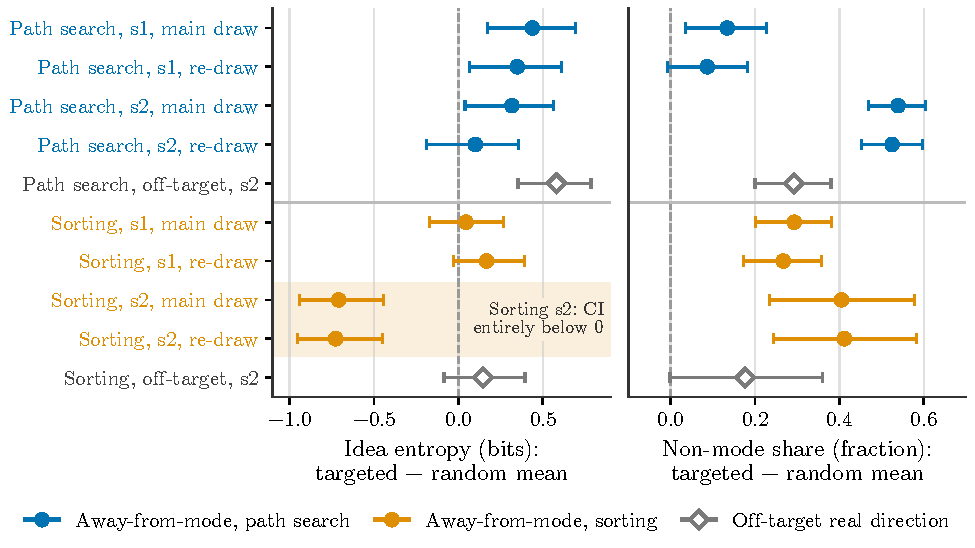
\includegraphics[width=\linewidth,height=0.85\textheight,keepaspectratio]{figures/fig3_v0.pdf}
  \caption{Preregistered comparisons of each targeted steering setting with the mean of five random directions of matched norm at the same strength (Qwen2.5-3B-Instruct; $n=150$ targeted generations per setting, 149 for the other task's direction on sorting; difference and 95\% hierarchical bootstrap CI as horizontal bars). Rows: the direction away from the mode at the lower ($s_1$) and higher ($s_2$) strength, on the main draw and on a redraw with fresh seeds, plus the other task's direction at $s_2$, for path search (blue) and sorting (orange). Filled circles are settings of the direction away from the mode, which we call away-from-mode in the plot legend, and hollow grey diamonds are the direction taken from the other task, which we call off-target in the plot labels. Dashed lines mark zero. Left: Miller--Madow idea entropy, targeted minus random mean (bits). Right: nonmodal share, which we call Non-mode share in the axis label (fraction of programs not implementing the baseline default), targeted minus random mean. Shaded band: on sorting at $s_2$, the direction away from the mode lowers entropy below the random mean on both draws, with the CI entirely below zero (selection), while raising the nonmodal share. On path search at $s_2$, the nonmodal share rises by more than 0.5 on both draws, while entropy rises less (main draw) or not detectably (redraw), because one family takes over. The other task's direction raises entropy on path search; on sorting, both of its intervals include zero.}
  \label{fig:forest}
\end{figure}

Three checks bound the result. First, the nearest neighbour ranking was wrong on both tasks: it predicted IDDFS for path search and selection sort for sorting. The direction lands on the family along its own projection, not on the family whose centroid lies closest to the mode. Second, the other task's direction also makes \Astar{} (26.7\%) and quicksort (34.7\%) the most common families other than the default, though neither reaches half the programs (the mode falls to 37.3\% and 23.3\%). \Astar{} is a common sink on path search: a negative instruction against greedy best first search also raises it, from 2.7\% to 58\% (Section~\ref{sec:res-context}). The predicted gainers are therefore partly the second most common family of each task, and the projection ranking's correct prediction is weaker evidence of geometric prediction than it first appears. Part of the effect is a generic push away from the default, and the task-specific direction is what turns it into a majority for one family. Third, random directions are not inert. On sorting, one random draw at $s_2$ gives selection sort 48\% of programs and another gives quicksort 50\%, and the random mode share at $s_2$ ranges from 0.19 to 0.69. Quicksort was also the most common nonmodal family in 7 of the 10 random cells on sorting, so on that task the identity of the gainer is less diagnostic than on path search, and the entropy contrast carries the evidence. A comparison with any single random cell would have misled in either direction.

\subsection{The same selection under a different prompt and layer band}
\label{sec:res-twofam}

A second experiment on the same model, with a different design, shows the same behaviour. There the prompt fixed the function signature and output format, which narrowed the path search menu to two families (BFS 98 and DFS 44 of 150 programs at temperature 0.7, pass rate 0.673), and the direction was a difference in means taken over the first 32 generated tokens at layers 29 to 31. The direction had been registered as a flattening control. At $\alpha = 0.224$ it produced DFS in 145 of 150 programs at an unchanged pass rate (0.680), and at $\alpha = 0.106$ already in 126. Idea entropy fell from 1.175 to 0.235 bits. Three random directions of matched norm at the same strength left the split near baseline (BFS 44 to 50, DFS 21 to 31 of 75).\footnote{Code: \url{https://github.com/ai-inventor-papers/ai-invention-8d19e3-temperature-flattens-ideas-context/tree/main/round-1/experiment-3}} With two families, a direction pointing from the mode toward the menu's mean overshoots the uniform point and selects the minority family. This measurement is exploratory as evidence for selection: the selection was observed after the flattening test it was designed for had failed. It agrees with the preregistered result on a different prompt, layer band and window.

\subsection{Selection does not reach new ideas}
\label{sec:res-offmenu}

If steering only selects among families the model already writes, it should fail to produce families it never writes. Table~\ref{tab:offmenu} tests this with directions toward the centroids of families outside the menu, built from programs the model wrote when asked for them, and compares them with simply asking.

\begin{table}[!htbp]
\centering
\caption{Steering toward a family outside the menu against naming it in the prompt: share of programs implementing the target family, and pass rate. Steered cells $n = 150$ at the frozen strengths ($\alpha = 0.224$, or $0.473$ for heap sort); prompted cells $n = 60$. Qwen2.5-3B-Instruct, temperature 0.7.}
\label{tab:offmenu}
\small
\begin{tabular}{@{}llrrrr@{}}
\toprule
 & & \multicolumn{2}{c}{Steered} & \multicolumn{2}{c}{Prompted} \\
\cmidrule(lr){3-4}\cmidrule(l){5-6}
Task & Target family & Target share & Pass & Target share & Pass \\
\midrule
Path search & IDDFS & 0.0\% & 0.30 & 91.7\% & 0.03 \\
Path search & Bellman-Ford & 0.0\% & 0.55 & 100\% & 0.75 \\
Sorting & Counting sort & 1.3\% & 0.98 & 100\% & 0.33 \\
Sorting & Heap sort & 91.3\% & 0.95 & 100\% & 1.00 \\
\bottomrule
\end{tabular}
\end{table}

Three of the four directions fail: the IDDFS direction moves mass from BFS to DFS (35.3\%) and the Bellman-Ford direction moves it to Dijkstra (34.7\%), the nearest families the model already writes. Heap sort is the exception, at 91.3\% with a pass rate of 0.95. Naming the family works for all four. The same holds for the broader notion of novelty. In the experiment with two families of Section~\ref{sec:res-twofam}, a blind judge labelled every passing program that the deterministic labeller had put in its residual class; all 70 were known algorithms. Asking for novelty in that experiment's prompt did no better: a request for a new algorithm left 136 of 150 path search programs on BFS or DFS, and a request for a fully novel algorithm of 2{,}000 words cut the pass rate from 0.67 to 0.11, with 65 programs DFS and 39 unparseable. The share of correct programs that implement no known algorithm was 0 in every condition of that experiment, including concept erasure with LEACE \citep{Belrose2023}, which cut the balanced accuracy of a linear idea probe on a weighted shortest path task from 0.888 to 0.334 (chance 0.333) without moving the outputs off the known families. On textbook tasks this metric is near its floor by construction, so the zero bounds novelty in this setting rather than in general.

\subsection{Temperature adds ideas slowly and breaks code quickly}
\label{sec:res-temp}

Figure~\ref{fig:temp} sets the number of families against correctness across temperature on the unsteered prompts. These cells come from the separate temperature sweep (vLLM, fresh seeds, 1{,}536-token cap), so their values differ slightly from the temperature rows of Table~\ref{tab:main}. On path search without top-$k$, the expected number of distinct families among ten programs moves from 3.48 at $T = 0.3$ to 3.91 at $T = 1.0$, while the pass rate falls from 0.49 to 0.19. At $T = 1.3$, 35\% of programs fall in the \emph{other} class and 65\% hit the token cap, and at $T = 1.6$ almost nothing parses. Sorting is the one task where heat buys ideas at little cost: the expected number of families among ten rises from 2.06 to 3.82 between $T = 0.3$ and $T = 1.0$ at a pass rate of 0.99, but the new mass goes to the same five comparison sorts. Top-$k$ 10 keeps $T = 1.6$ parseable and adds a few rare families (nine classes on path search), at a pass rate of 0.06 on path search and 0.82 on sorting. On the weighted shortest path prompt the model writes Dijkstra's algorithm in 98 to 100 of 100 programs up to $T = 1.0$.

\begin{figure}[!htbp]
  \centering
  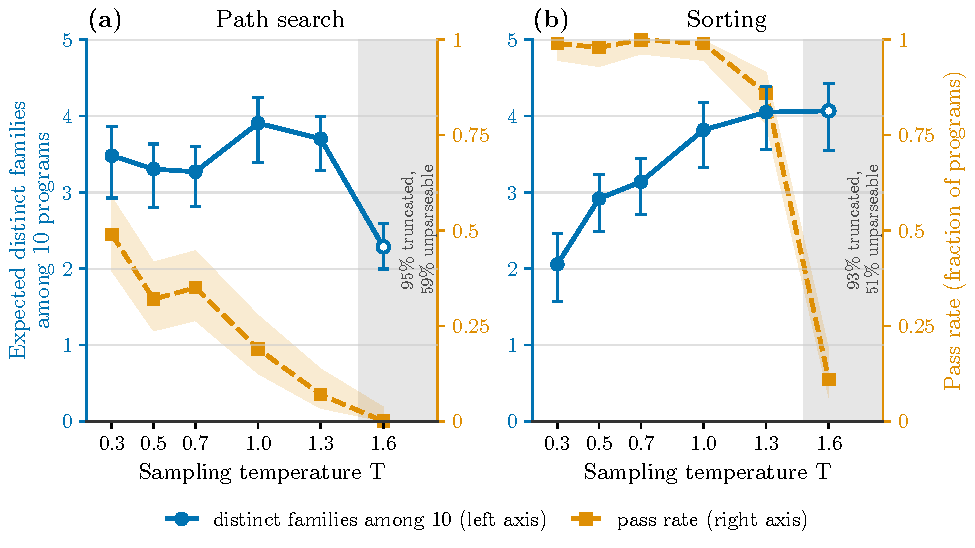
\includegraphics[width=\linewidth,height=0.85\textheight,keepaspectratio]{figures/fig4_v0.pdf}
  \caption{Expected number of distinct algorithm families among ten programs (blue solid line, circles, left axis; error bars are 95\% multinomial bootstrap intervals over the label counts) and oracle pass rate (amber dashed line, squares, right axis; shaded band is the Wilson 95\% interval) against sampling temperature $T$, without top-$k$, for Qwen2.5-3B-Instruct on the bare path search (a) and sorting (b) prompts; $n = 100$ programs per temperature, fresh seeds, 1{,}536-token cap. On path search the family count stays between 3.27 and 3.91 up to $T = 1.3$ while the pass rate falls from 0.49 at $T = 0.3$ to 0.07. On sorting, heat raises the family count from 2.06 to 4.05 by $T = 1.3$, as Bubble sort's share drops from 88\% to 41\% in favour of Quick, Merge and Insertion sort, at a pass rate still of 0.86. Code then collapses at $T = 1.6$, where the pass rate is 0.11. In the grey $T = 1.6$ column, 95\% (a) and 93\% (b) of outputs hit the token cap and 59\% and 51\% are labelled unparseable. The family count there (hollow circle) counts the \emph{Unparseable} and \emph{Other} labels as families and is not real algorithmic variety. Idea count changes little relative to the collapse in correctness.}
  \label{fig:temp}
\end{figure}

The model's default is a mode, not an average. Even at $T = 0.3$ with top-$k$ 10, ten path search programs contain about 3.5 ideas written in about 9 distinct phrasings; the case of ten ideas with one phrasing each never occurs in any cell (the largest expected count among ten is 4.9). A preregistered law in which temperature only rescales fixed idea utilities, so that idea log odds are linear in $1/T$ without reordering, failed its criteria on both tasks and both draws. Out of sample it beat a fixed utility baseline (the $T = 0.7$ shares raised to the power $0.7/T$) on path search (mean absolute error 0.040 against 0.073) but lost on sorting (0.100 against 0.028). Raising temperature is a weak way to change the idea and a strong way to lose correctness.

\subsection{Prompt context also selects rather than diversifies}
\label{sec:res-context}

Two manipulations of the prompt behave like the steering direction. Prepending a random seed string in the format of \texttt{seed=d32qxk4nt43} (60 strings of random characters such as \texttt{seed=i9609s2lg7o} and 60 lists of four random words such as \texttt{seed=(mask bed square finger)}; the two literal example strings were not among them) to the prompt lowers idea entropy at $T = 0.7$ by 0.34 bits on path search ([$-0.53$, $-0.13$]) and 0.68 bits on sorting ([$-0.92$, $-0.47$]), over 120 strings with 5 samples each against 300 unseeded programs. On sorting, random words send 282 of 300 programs to bubble sort. In the last five layers the strings displace the residual stream at the final prompt tokens 2.6 to 3.2 times as much as a negative instruction does, so a large internal displacement in an irrelevant direction concentrates the choice instead of spreading it. This narrowing is an exploratory finding: the preregistered prediction of seed effects from a utility gap failed (sorting predicted flip rate 0.39, observed 0.017).

Negative instructions (\emph{Do not use X.} appended to the prompt) act as instructions to choose something else rather than as removal of an option. The comparison condition is a placebo prompt, that is, a prompt that appends a negative instruction against an irrelevant algorithm (\emph{Do not use the Rabin-Karp algorithm.} for path search, \emph{Do not use Kruskal's algorithm.} for sorting). In a preregistered test on 5{,}930 confirmation programs generated after all predictors were frozen, negative instructions lowered the share of a family they did not name, which pure restriction of the choice set cannot do, in 8 of 46 tested cells (Fisher's exact test with Holm correction, $p < 0.01$, drop larger than the placebo noise floor), spread over 6 negative instructions. Placebo blocks compared with each other gave 0 such cells out of 45, and shuffling the labels of negative-instruction and placebo programs gave 0 in each of 20 repetitions.\footnote{Code: \url{https://github.com/ai-inventor-papers/ai-invention-8d19e3-temperature-flattens-ideas-context/tree/main/round-2/experiment-5}} Table~\ref{tab:ban} lists the clearest cases, which are negative instructions against families the model almost never writes, and Figure~\ref{fig:ban} plots them.

\begin{table}[!htbp]
\centering
\caption{A negative instruction against a family the model almost never writes moves the families it does write (Qwen2.5-3B-Instruct, $n = 100$ per negative instruction, placebo $n = 300$; \% of programs).}
\label{tab:ban}
\small
\begin{tabularx}{\linewidth}{@{}lYYY@{}}
\toprule
Task & Banned family (placebo share) & Mode, placebo $\to$ banned & Largest gainer, placebo $\to$ banned \\
\midrule
Path search & greedy best first (0\%) & BFS 63.3 $\to$ 23.0 & \Astar{} 2.7 $\to$ 58.0 \\
Path search & IDDFS (0\%) & BFS 63.3 $\to$ 41.0 & \Astar{} 2.7 $\to$ 49.0 \\
Path search & Bellman-Ford (0\%) & BFS 63.3 $\to$ 40.0 & Dijkstra 4.7 $\to$ 56.0 \\
Sorting & radix sort (0\%) & bubble 54.0 $\to$ 15.0 & merge 15.0 $\to$ 39.0 \\
Sorting & counting sort (0\%) & bubble 54.0 $\to$ 26.0 & quick 18.0 $\to$ 35.0 \\
Sorting & shell sort (0\%) & bubble 54.0 $\to$ 28.0 & merge 15.0 $\to$ 49.0 \\
\bottomrule
\end{tabularx}
\end{table}

\begin{figure}[!htbp]
  \centering
  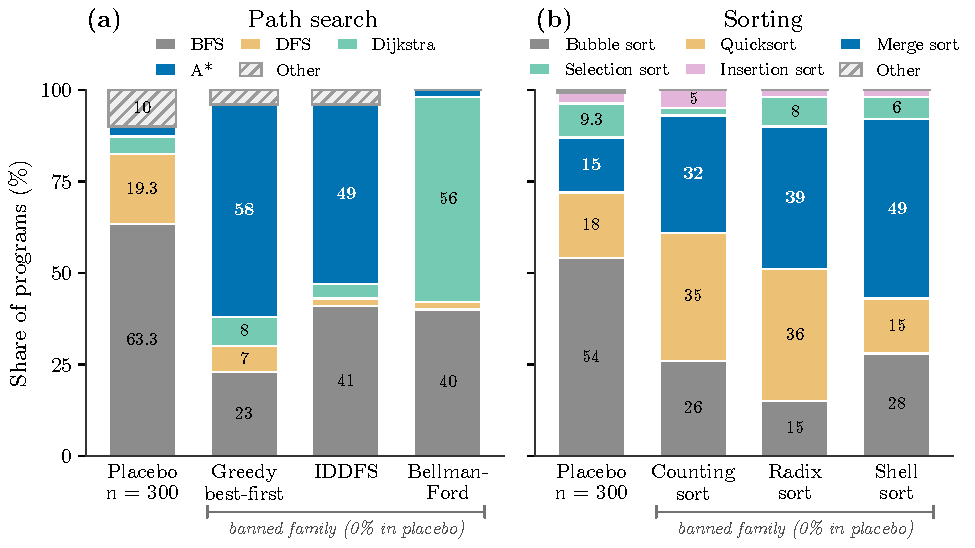
\includegraphics[width=\linewidth,height=0.85\textheight,keepaspectratio]{figures/fig5_v0.pdf}
  \caption{Share of programs per algorithm family written by Qwen2.5-3B-Instruct, on (a) path search and (b) sorting. In each panel, the first bar is a placebo prompt, a negative instruction against an irrelevant algorithm (pooled over three placebo cells, $n=300$). The other three bars are negative instructions against a family the model writes in 0\% of placebo programs ($n=100$ each; bracket: \emph{banned family (0\% in placebo)}). All programs were generated after the predictors were frozen. Each bar is a 100\%-stacked composition. The vertical axis gives the share of programs (\%) and segment labels give that share for segments of 5\% or more. Grey is the default family (BFS; bubble sort), blue is A* and merge sort, amber is DFS and quicksort, green is Dijkstra and selection sort, pink is insertion sort, and hatched light grey is all other labels (including SPFA, heap sort, unparseable programs and the 1\% of programs that still use the banned family). Banning greedy best first search sends A* from 2.7\% to 58\% and BFS from 63.3\% to 23\%. Banning Bellman-Ford sends Dijkstra from 4.7\% to 56\%. Banning radix sort cuts bubble sort from 54\% to 15\% while merge sort rises from 15\% to 39\%. Bars show single cells without error bars. Of the 46 drops (one family under one negative instruction) tested with Fisher's exact test and Holm correction, 8 are significant, against 0 of 45 in comparisons of placebo against placebo. Restricting the choice set alone cannot lower the share of a family that remains available, so these drops mean the negative instruction reweights the remaining families rather than only removing an option.}
  \label{fig:ban}
\end{figure}

The internal account of negative instructions is partial. We call the \emph{displacement} of a negative instruction the difference between its residual stream activations at the final prompt tokens and those of the placebo prompt. The displacement predicts the sign of share changes in 83\% of cells where an idea moved by at least 10 points, against 65\% for proportional renormalisation (independence of irrelevant alternatives, IIA). It reduces the Jensen--Shannon divergence to the observed distribution by only 9.2\% relative to IIA ([$-0.6$\%, 19.6\%], 20\% required). Adding that displacement to a placebo run recovers none of the effect (mean recovery $-0.001$, against $-0.006$ for random displacements; recovery is one minus the ratio of the divergence after patching to the divergence before). In contrast, an attention knockout from generated tokens to the negative-instruction sentence during decoding restores the placebo distribution (mean restoration 0.72 over four negative instructions, where restoration is the matching quantity for removing the effect from the negative-instruction run; an exploratory manipulation). The logit lens of the displacement shows tokens such as \emph{while}, \emph{another} and \emph{rather} and ranks the banned name about 17{,}600th (median over 27 negative instructions), so the final prompt state reads as an instruction to do something else rather than as priming of the named family. On gemma-2-2b-it, regularity violations were rare (1 of 72 cells) and the displacement predictor lost to IIA (mean divergence 0.121 against 0.088).

\section{Discussion}
\label{sec:discussion}

Across four kinds of control, the model behaves as if it holds a short ranked list of textbook ideas for each prompt and returns its top entry. Activation steering along the direction away from the mode moves the top of that list to a predictable second entry. Negative instructions move it to a particular other entry, even when the banned family was never on the list. Seed strings make the top entry more dominant. Temperature reaches lower entries slowly while breaking the code. None of them adds an entry. This pattern answers the practitioner's question in a specific way: on these tasks, the controls that change the solution idea are controls of \emph{which known idea}, and the control that reaches an unlisted idea is the plain instruction to use it.

The distinction between selecting and flattening matters for how steering for diversity is evaluated. On path search, entropy rose under steering, and an evaluation that scored diversity by entropy against a single random direction would have reported a diversity gain. The view at the level of families shows a switch from one default to another, with the pass rate halved. The random baseline averaged over draws was necessary in the other direction too: individual random draws produced shifts that resemble selection on sorting, so a single random comparator could have made the targeted direction look either unremarkable or exceptional. Two practices follow for steering studies that claim diversity or creativity gains: report what fraction of the gain goes to one family, and compare with the mean of several random directions of matched norm rather than one.

The results agree with reports that steering reliability varies by concept and input \citep{Tan2024} and that prompting often matches steering \citep{Wu2025}; Table~\ref{tab:offmenu} is an instance of the latter for ideas outside the menu. They do not contradict reports that jointly optimised directions diversify concurrent generations \citep{Zhu2026,Khanh2025}, which is a different intervention, or that a direction from boring to creative activations raises the creativity of text \citep{Olson2024}, which was measured on open prose. In the experiment with two families, a direction separating prompts that request a novel algorithm from plain prompts, built on other tasks, transferred perfectly as a readout of whether novelty was requested (AUROC 1.0), but its effect on atypicality was not monotone in strength (Spearman 0.49 and $-0.26$). Reading a concept and moving behaviour along it are separate properties.

Two questions practitioners ask about sampling and negative instructions have direct answers in these data. First, at a low temperature with top-$k$ 10, ten samples hold a few ideas in many phrasings, not many ideas in one phrasing each; raising temperature adds phrasings quickly and ideas slowly. Second, we asked whether, after the most common families are banned, mass moves to the edge of the banned region of representation space or to its far side. We call the \emph{edge statistic} the difference between the internal similarity of the post-ban idea mass to the banned ideas' centroids and the similarity the placebo mass would give; positive values mean mass lands near the banned ideas. On the initial set of negative instructions it is positive for most path search cases (0.14 to 0.29) and has no consistent sign on sorting, and when the top five families are banned it is near zero on path search, sorting and weighted shortest path ($-0.035$, 0.006, 0.003). In a principal component projection of activations over the commitment window, the idea label explains 77\% of the variance of the first component on path search, which separates shortest path methods (Dijkstra, Bellman-Ford, Floyd-Warshall) from unweighted searches (BFS, DFS, IDDFS); the second separates heuristic searches (\Astar{}, greedy best first, bidirectional). The direction away from the mode lands on \Astar{}, at the heuristic end, rather than on IDDFS, the nearest neighbour of BFS.

\section{Limitations}
\label{sec:limitations}

The selection result is measured on one model, Qwen2.5-3B-Instruct, and two prompts, each with one wording. The SELECT rule accepted the top prediction of either of two frozen rankings, which loosens it, and on path search the $s_2$ operating point missed the frozen pass-rate bar (0.17 against 0.25). The steering test was not run on gemma-2-2b-it, and the negative-instruction results there did not reproduce the Qwen pattern, so the claim does not extend to other families or scales without new evidence. The layer band was chosen by a probe whose accuracy was flat across layers, and the window covers the first 64 generated tokens; other bands or windows may flatten where this one selects.

On path search, the labeller agrees with a blind judge at kappa 0.39 on steered outputs, so the exact \Astar{} share is uncertain even though its rise from 8\% to 57\% and 63\% far exceeds that error; the sorting result, at kappa 0.94, is the cleaner of the two. Steering on path search halved the pass rate and pushed 77\% to 78\% of outputs to the token cap, so selection there comes with a correctness cost the frozen calibration did not predict. Truncation also affects labels: continuing 150 truncated programs flipped 10.7\% of labels in the temperature experiments, and batch composition alone flips 11\% to 17\% of labels in repeated runs.

Novelty was measured as correct code outside known algorithm families, which is near zero by construction on textbook tasks. Only the experiment with two families had a judge check the passing programs in the labeller's residual class; 11 such programs from the later experiments were not judged. The result says that these controls did not create new algorithms for path search and sorting, not that steering cannot raise novelty on open problems. The experiment with two families of Section~\ref{sec:res-twofam} is exploratory evidence for selection, and the seed narrowing, the attention knockout and the edge statistic are exploratory too. The point at which the model commits to an idea is not located: probes on the first eight generated tokens were at chance, and neither forking-path resampling \citep{Bigelow2024} nor other attribution of individual tokens by resampling was run. The manifold of idea centroids is reported only through the principal component statistics of Section~\ref{sec:discussion}, without a figure. A sparse autoencoder analysis on gemma-2-2b-it with Gemma Scope dictionaries \citep{Lieberum2024} reconstructed activations poorly (fraction of variance unexplained 0.61) and supports no claim.

\section{Conclusion}
\label{sec:conclusion}

A difference-in-means direction away from a code model's default algorithm does not spread probability across the algorithms the model knows; it hands the default's share to one predicted second choice. On sorting, quicksort rose to 68\% of programs and entropy fell 0.73 bits below matched random directions on a redraw with fresh seeds under frozen rules, and path search shifted from BFS to \Astar{} at 57\% and 63\%. Steering toward algorithms the model never writes failed where a request of one sentence succeeded, and every passing program outside the labelled families that a judge checked was a textbook algorithm. Temperature, seed strings and negative instructions likewise reorder or concentrate a short menu. Future work should:
\begin{itemize}
  \item test the rule that separates selecting from flattening on other model families and sizes, and on tasks without a textbook menu;
  \item locate where the idea is fixed during generation, with forking-path resampling and attention-head patching around the negative-instruction sentence;
  \item report concentration at the level of families next to entropy whenever steering is evaluated for diversity.
\end{itemize}

\paragraph{Code and data availability.} All code, generations and analysis outputs behind the reported numbers are public at \url{https://github.com/ai-inventor-papers/ai-invention-8d19e3-temperature-flattens-ideas-context}; the footnotes in Sections~\ref{sec:setup} and~\ref{sec:results} point to the experiment behind each result.

\bibliographystyle{plainnat}
\bibliography{references}

\end{document}
